%%\documentclass[a4paper,12pt,oneside]{llncs}
\documentclass{book}
%\usepackage[right=2cm,left=3cm,top=2cm,bottom=2cm,headsep=0cm]{geometry}

%%%%%%%%%%%%%%%%%%%%%%%%%%%%%%%%%%%%%%%%%%%%%%%%%%%%%%%%%%%
%% Juego de caracteres usado en el archivo fuente: UTF-8
\usepackage{ucs}
\usepackage[utf8]{inputenc}
\usepackage{eurosym}

%%%%%%%%%%%%%%%%%%%%%%%%%%%%%%%%%%%%%%%%%%%%%%%%%%%%%%%%%%%
%% Juego de caracteres usado en la salida dvi
%% Otra posibilidad: \usepackage{t1enc}
\usepackage[T1]{fontenc}

%%%%%%%%%%%%%%%%%%%%%%%%%%%%%%%%%%%%%%%%%%%%%%%%%%%%%%%%%%%
%% Ajusta maergenes para a4
\usepackage{a4wide}

%%%%%%%%%%%%%%%%%%%%%%%%%%%%%%%%%%%%%%%%%%%%%%%%%%%%%%%%%%%
%% Uso fuente postscript times, para que los ps y pdf queden y pequeños...
\usepackage{times}

%%%%%%%%%%%%%%%%%%%%%%%%%%%%%%%%%%%%%%%%%%%%%%%%%%%%%%%%%%%
%% Posibilidad de hipertexto (especialmente en pdf)
\usepackage{hyperref}

%%%%%%%%%%%%%%%%%%%%%%%%%%%%%%%%%%%%%%%%%%%%%%%%%%%%%%%%%%%
%% Graficos 
\usepackage{graphics,graphicx}

%%%%%%%%%%%%%%%%%%%%%%%%%%%%%%%%%%%%%%%%%%%%%%%%%%%%%%%%%%%
%% Ciertos caracteres "raros"...
\usepackage{latexsym}

%%%%%%%%%%%%%%%%%%%%%%%%%%%%%%%%%%%%%%%%%%%%%%%%%%%%%%%%%%%
%% Matematicas aun más fuertes (american math dociety)
\usepackage{amsmath}

%%%%%%%%%%%%%%%%%%%%%%%%%%%%%%%%%%%%%%%%%%%%%%%%%%%%%%%%%%%
%\usepackage{multirow} % para las tablas
%\usepackage[spanish,es-tabla]{babel}

%%%%%%%%%%%%%%%%%%%%%%%%%%%%%%%%%%%%%%%%%%%%%%%%%%%%%%%%%%%
%% Fuentes matematicas lo mas compatibles posibles con postscript (times)
%% (Esto no funciona para todos los simbolos pero reduce mucho el tamaño del
%% pdf si hay muchas matamaticas....
\usepackage{mathptm}

%%% VARIOS:
%\usepackage{slashbox}
\usepackage{verbatim}
\usepackage{array}
\usepackage{listings}
\usepackage{multirow}
\usepackage{hhline}

%% MARCA DE AGUA
%% Este package de "draft copy" NO funciona con pdflatex
%%\usepackage{draftcopy}
%% Este package de "draft copy" SI funciona con pdflatex
%%%\usepackage{pdfdraftcopy}
%%%%%%%%%%%%%%%%%%%%%%%%%%%%%%%%%%%%%%%%%%%%%%%%%%%%%%%%%%%
%% Indenteacion en español...
\usepackage[spanish,USenglish]{babel}
\usepackage{Estilos/Apuntes}
\usepackage[svgnames,x11names,table]{xcolor}
\usepackage{listings}
% Para escribir código en C
% \begin{verbatim}[language=C]
% #include <stdio.h>
% int main(int argc, char* argv[]) {
% puts("Hola mundo!");
% }
% \end{verbatim}



%%Configuracion del paquete listings
\lstset{language=bash, numbers=left, numberstyle=\tiny, numbersep=10pt, firstnumber=1, stepnumber=1}

\begin{document}
	\begin{titlepage}
		\centering
		
		{\scshape\huge University of Cádiz \par}
		\vspace{1cm}
		{\scshape\LARGE Faculty of Engeneering\par}
		\vspace{1cm}
		{\scshape\Large{Stimey}\par}
		\vspace{1cm}
		{\Huge\bfseries Fantasy\par}
		\vspace{1cm}
		{\Large\itshape Luis Gutiérrez Flores\\
			Nicolás Ruiz Requejo\\
			Jesús Rodríguez Heras\\
			Arantzazu Otal Alberro\\
			Alejandro Segovia Gallardo\\
			Alejandro José Caraballo García\\
			Gabriel Fernando Sánchez Reina\par}
		\vspace{2.5cm}
		\begin{table}[htb]
			\centering
			\begin{tabular}{ccc}
				
\includegraphics[width=0.15\textwidth]{UCA.png}\par\vspace{1.2cm} & 
\includegraphics[width=0.15\textwidth]{ESI.png}\par\vspace{1.2cm} & 
\includegraphics[width=0.15\textwidth]{Stimey.png}\par\vspace{1.2cm}
			\end{tabular}
		\end{table}
		%		\vfill
		
		
		
		% Bottom of the page
		%		{\large \today\par}
	\end{titlepage}

	\tableofcontents
	\newpage
	
	\chapter{Analisys of requirements}
\section{Agents catalogue}
Fantasy project agents catalogue will be the students who interact with de webpage.

These agents can be sorted in two groups: students and teachers.

\subsection{Teachers}
\begin{itemize}
	\item \textbf{Background:} They can open a window where you can select an image from the Internet, the computer or an image previously used. This image will cover all the workspace.
	\item \textbf{Active Point:} They can establish active points in the workspace and modify them conveniently by adding images, text, video, audio, etc. They can also establish a score for each active point of the fantasy to evaluate the students.
\end{itemize}

\subsection{Students}
\begin{itemize}
	\item \textbf{Background:} They can do the same as the teachers.
	\item \textbf{Active Point:} They can establish active points in the workspace and modify them conveniently by adding images, text, video, audio, etc. You can not set a score for active points.
\end{itemize}

\section{Functional requiriments}
All the use cases described below have the following implicit precondition to be able to use said use cases in the final application:
\begin{itemize}
	\item The user (teachers/students) must have an account on the STIMEY platform and have logged in with that account.
\end{itemize}

The proposed use cases are the following:

\subsection{CRUD fantasy}
\hypertarget{crearfantasia}{}
\subsubsection{Use case: Create fantasy}
\begin{itemize}
	\item \textbf{Description:} Create a new fantasy.
	\item \textbf{Agents:} Creator-editor (user).
	\item \textbf{Preconditions:} The user must have permission to create a new fantasy.
	\item \textbf{Postconditions:} Fantasy is stored in the system.
	\item \textbf{Main stage:}
	\begin{enumerate}
		\item The user selects the option ``Create new fantasy''.
		\item The system requests the name of the fantasy.
		\item The user enters the name of the fantasy.
		\item The system requests the fantasy code.
		\item The user enters the fantasy code.
		\item The system gives you the option to choose if the fantasy will be public (by default), shared or private.
		\item The user selects `` Public ''.
		\item The user creates the fantasy.
		\item The fantasy is stored in the system.
	\end{enumerate}
	\item \textbf{Extensions:} \\7. a) The user selects that the fantasy will be shared.
	\begin{enumerate}
		\item The system allows to insert in a list the identifiers of other users with which the fantasy will be shared.
		\item The user enters the identifiers of the users who will share the fantasy.
		\item Step 8.
	\end{enumerate}
	7. b) The user selects that the fantasy will be private.
	\begin{enumerate}
		\item The system marks the fantasy as private for that user without giving the possibility of sharing.
		\item Step 8.
	\end{enumerate}
	*a) At any time, the user can go back to the main menu.
	\item \textbf{Variations:} None.
	\item \textbf{Not-functional:} None.
	\item \textbf{Issues:} None.
\end{itemize}

\subsubsection{Use case: Visualize fantasy}
\begin{itemize}
	\item \textbf{Description:} Read an existing fantasy.
	\item \textbf{Agents:} Creator-editor (user).
	\item \textbf{Preconditions:} The fantasy must exist in the system and the user must have the modification permissions.
	\item \textbf{Postconditions:} There are no changes in the fantasy.
	\item \textbf{Main stage:}
	\begin{enumerate}
		\item The user selects the option ``My fantasies''
		\item The system displays a list of fantasies accessible by the user.
		\item The user selects the fantasy that he wants to visualize.
		\item The system displays a pop-up window with the fantasy information and its options.
		\item The user selects the option ``Visualize fantasy''.
		\item The system shows the fantasy.
		\item The user reads the fantasy without making any changes and, when it is over, closes the fantasy.
		\item The fantasy remains unchanged.
	\end{enumerate}
	\item \textbf{Extensions:} \\ *a) At any time, the user can go back to the main menu.
	\item \textbf{Variations:} None.
	\item \textbf{Not-functional:} None.
	\item \textbf{Issues:} None.
\end{itemize}

\subsubsection{Use case: Update fantasy}
\begin{itemize}
	\item \textbf{Description:} Modify an existing fantasy.
	\item \textbf{Agents:} Creator-editor (user).
	\item \textbf{Preconditions:} The fantasy must exist in the system and the user must have the modification permissions.
	\item \textbf{Postconditions:} The fantasy is modified.
	\item \textbf{Main stage:}
	\begin{enumerate}
		\item The user selects the option ``My fantasies''.
		\item The system displays a list of fantasies accessible by the user.
		\item The user selects the fantasy that he wants to modify.
		\item The system displays a pop-up window with the fantasy information and its options.
		\item The user selects the option ``Modify fantasy''.
		\item The system displays the fantasy creation screen for modification.
	\end{enumerate}
	\item \textbf{Extensions:} \\ *a) At any time, the user can go back to the main menu.
	\item \textbf{Variations:} None.
	\item \textbf{Not-functional:} None.
	\item \textbf{Issues:} None.
\end{itemize}

\subsubsection{Use case: Delete fantasía}
\begin{itemize}
	\item \textbf{Description:} Erase an existing fantasy.
	\item \textbf{Agents:} Creator-editor (user).
	\item \textbf{Preconditions:} The fantasy must exist in the system and the user must have the removal permissions.
	\item \textbf{Postconditions:} Fantasy is eliminated from the system.
	\item \textbf{Main stage:}
	\begin{enumerate}
		\item The user selects the option ``My fantasies''.
		\item The system displays a list of fantasies accessible by the user.
		\item The user selects the fantasy that he wants to modify.
		\item The system displays a pop-up window with the fantasy information and its options.
		\item The user selects the option ``Clear fantasy''.
		\item The system displays a confirmation message.
		\item The user selects ``Accept''.
		\item The system erases the fantasy.
	\end{enumerate}
	\item \textbf{Extensions:}  \\7. a) The user selects ``Cancel''.
	\begin{enumerate}
		\item The system closes the pop-up window.
		\item Step 1.
	\end{enumerate}
	*a) At any time, the user can go back to the main menu.
	\item \textbf{Variations:} None.
	\item \textbf{Not-functional:} None.
	\item \textbf{Issues:} None.
\end{itemize}

\subsection{Use case: Copy fantasy}
\begin{itemize}
	\item \textbf{Description:} Clone a fantasy.
	\item \textbf{Agents:} Creator-editor (user).
	\item \textbf{Preconditions:} The fantasy must exist in the system and the user must have the modification permissions.
	\item \textbf{Postconditions:} Create a copy of the selected fantasy.
	\item \textbf{Main stage:}
	\begin{enumerate}
		\item The user selects the option ``My fantasies''.
		\item The system displays a list of fantasies accessible by the user.
		\item The user selects the fantasy that he wants to copy.
		\item The system displays a pop-up window with the fantasy information and its options.
		\item The user selects the option ``Copy fantasy''.
		\item The system creates a copy of the selected fantasy.
	\end{enumerate}
	\item \textbf{Extensions:} \\ *a) At any time, the user can go back to the main menu.
	\item \textbf{Variations:} None.
	\item \textbf{Not-functional:} None.
	\item \textbf{Issues:} None.
\end{itemize}

\subsection{CRUD background}
\begin{itemize}
	\item \textbf{Description:} Allows selecting, modifying and deleting the background.
	\item \textbf{Agents:} Creator-editor (user).
	\item \textbf{Preconditions:} The fantasy must exist in the system and the user must have the modification permissions.
	\item \textbf{Postconditions:} The background that the user has chosen is established.
	\item \textbf{Main stage:}
	\begin{enumerate}
		\item The user selects the ``Background'' option.
		\item The system displays a window to add a background to the workspace.
		\item The user selects an image.
		\item The system sets the background selected by the user.
	\end{enumerate}
	\item \textbf{Extensions:} \\ *a) At any time, the user can go back to the main menu. 
	\item \textbf{Variations:} None.
	\item \textbf{Not-functional:} None.
	\item \textbf{Issues:} None.
\end{itemize}


\subsection{CRUD active point}
\subsubsection{Use case: Create active point}
\begin{itemize}
	\item \textbf{Description:} Create a new active point.
	\item \textbf{Agents:} Creator-editor (user).
	\item \textbf{Preconditions:} The fantasy must exist in the system and the user must have the modification permissions.
	\item \textbf{Postconditions:} An empty active point is created in the workspace.
	\item \textbf{Main stage:}
	\begin{enumerate}
		\item The user selects the option ``New active point''.
		\item The system creates a new active point in the workspace.
		\item The user can move the active point to the area of the workspace that he wants.
		\item The system will save the active point in the fantasy.
	\end{enumerate}
	\item \textbf{Extensiones:} \\ *a) At any time, the user can go back.
	\item \textbf{Variations:} None.
	\item \textbf{Not-functional:} None.
	\item \textbf{Issues:} None.
\end{itemize}

\subsubsection{Use case: Visualize active point}
\begin{itemize}
	\item \textbf{Description:} Shows an existing active point for reading.
	\item \textbf{Agents:} Creator-editor (user).
	\item \textbf{Preconditions:} Fantasy must exist in the system and the active point must exist in fantasy. In addition, the user must have the modification permissions.
	\item \textbf{Postconditions:} The active point is shown for reading.
	\item \textbf{Main stage:}
	\begin{enumerate}
		\item The user selects the active point that he wants to view.
		\item The system displays a window with the information of the active point and its options.
		\item The user selects the option ``Visualize''.
		\item The system displays a window with the summary of that active point.
	\end{enumerate}
	\item \textbf{Extensions:} \\ *a) At any time, the user can go back.
	\item \textbf{Variations:} None.
	\item \textbf{Not-functional:} None.
	\item \textbf{Issues:} None.
\end{itemize}

\subsubsection{Use case: Update active point}
\begin{itemize}
	\item \textbf{Description:} Modifies an existing active point.
	\item \textbf{Agents:} Creator-editor (user).
	\item \textbf{Preconditions:} Fantasy must exist in the system and the active point must exist in fantasy. In addition, the user must have the modification permissions.
	\item \textbf{Postconditions:} Modifies the selected active point.
	\item \textbf{Main stage:}
	\begin{enumerate}
		\item The user selects the active point that he wants to modify.
		\item The system displays a window with the information of the active point and its options.
		\item The user selects the option ``Modify''.
		\item The system displays the creation window of the active point.
	\end{enumerate}
	\item \textbf{Extensions:} \\ *a) At any time, the user can go back.
	\item \textbf{Variations:} None.
	\item \textbf{Not-functional:} None.
	\item \textbf{Issues:} None.
\end{itemize}

\subsubsection{Use case: Delete active point}
\begin{itemize}
	\item \textbf{Description:} Deletes an existing active point.
	\item \textbf{Agents:} Creator-editor (user).
	\item \textbf{Preconditions:} Fantasy must exist in the system and the active point must exist in fantasy. In addition, the user must have the modification permissions.
	\item \textbf{Postconditions:} Deletes the selected active point.
	\item \textbf{Main stage:}
	\begin{enumerate}
		\item The user selects the active point that he wants to delete.
		\item The system displays a window with the information of the active point and its options.
		\item The user selects the option ``Delete''.
		\item The system displays a confirmation message.
		\item The user selects ``Accept''.
		\item The system deletes the active point.
	\end{enumerate}
	\item \textbf{Extensions:} \\ 5. a) The user selects ``Cancel''.
	\begin{enumerate}
		\item The system closes the pop-up window.
		\item Step 1.
	\end{enumerate}
	*a) At any time, the user can go back.
	\item \textbf{Variations:} None.
	\item \textbf{Not-functional:} None.
	\item \textbf{Issues:} None.
\end{itemize}

\subsection{CRUD image}
\hypertarget{crearimagen}{}
\subsubsection{Use case: Create image}
\begin{itemize}
	\item \textbf{Description:} Insert an image in an active point.
	\item \textbf{Agents:} Creator-editor (user).
	\item \textbf{Preconditions:} The corresponding active point must exist and the fantasy must be being edited.
	\item \textbf{Postconditions:} Insert an image in the selected active point.
	\item \textbf{Main stage:}
	\begin{enumerate}
		\item The user selects the corresponding active point within the fantasy.
		\item The system displays a pop-up window with the information of the active point.
		\item The user selects the option ``Insert image''.
		\item The system shows a window in which the user chooses from where they can insert the image (Internet, local, image already used in fantasy).
		\item The user chooses the option ``Internet'' to include an image of the Internet.
		\item The system asks the user for the url of the image.
		\item The user inserts the correct url of the image.
		\item The active point takes the shape of the image.
	\end{enumerate}
	\item \textbf{Extensions:} \\5. a) The user chooses the ``Local'' option to include an image from his computer.
	\begin{enumerate}
		\item The system opens a file browser window.
		\item The user selects the image and press ``Accept''.
		\item The system closes the file browser window.
		\item Step 8.
	\end{enumerate}
	5. b) The user chooses the option ``Image previously used'' to include an image previously used.
	\begin{enumerate}
		\item The system opens a window with the images previously used.
		\item The user selects the image and press ``Accept''.
		\item The system closes the pop-up window.
		\item Step 8.
	\end{enumerate}
	7. a) The url is not correct.
	\begin{enumerate}
		\item The system displays an error message.
		\item Step 6.
	\end{enumerate}
	*a) At any time, the user can go back.
	\item \textbf{Variations:} None.
	\item \textbf{Not-functional:} None.
	\item \textbf{Issues:} None. %Ya dijimos que si podía, con el pixlr
\end{itemize}

\subsubsection{Use case: Update image}
\begin{itemize}
	\item \textbf{Description:} Update an image.
	\item \textbf{Agents:} Creator-editor (user).
	\item \textbf{Preconditions:} There must exists the corresponding active point, you must be editing the fantasy and there must be an image.
	\item \textbf{Postconditions:} The image is modified.
	\item \textbf{Main stage:}
	\begin{enumerate}
		\item The user selects the corresponding active point within the fantasy.
		\item The system opens a popup window with the information of the active point.
		\item Step 4 of \hyperlink{crearimagen}{Create image}.
	\end{enumerate}
	\item \textbf{Extensiones:} \\ *a) At any time, the user can go back.
	\item \textbf{Variations:} None.
	\item \textbf{Not-functional:} None.
	\item \textbf{Issues:} None.
\end{itemize}

\subsubsection{Use case: Delete image}
\begin{itemize}
	\item \textbf{Description:} Delete an image of an active point.
	\item \textbf{Agents:} Creator-editor (user).
	\item \textbf{Preconditions:} There must be the corresponding active point, you must be editing the fantasy and there must be an image.
	\item \textbf{Postconditions:} Delete the image and leave the active point in its default state.
	\item \textbf{Main stage:}
	\begin{enumerate}
		\item The user selects the corresponding active point within the fantasy.
		\item The system opens a popup window with the information of the active point.
		\item The user selects the image and presses the ``Delete'' button.
		\item The system displays a confirmation message.
		\item The user selects ``Accept''.
		\item The system deletes the image of the active point.
	\end{enumerate}
	\item \textbf{Extensions:} \\ 5. a) The user selects ``Cancel''.
	\begin{enumerate}
		\item The system closes the pop-up window.
		\item Step 1.
	\end{enumerate}
	*a) At any time, the user can go back.
	\item \textbf{Variations:} None.
	\item \textbf{Not-functional:} None.
	\item \textbf{Issues:} None.
\end{itemize}

\subsection{CRUD video}
\hypertarget{crearvideo}{}
\subsubsection{Use case: Create video}
\begin{itemize}
	\item \textbf{Description:} Insert a video in an active point.
	\item \textbf{Agents:} Creator-editor (user).
	\item \textbf{Preconditions:} The corresponding active point must exist and the fantasy must be being edited.
	\item \textbf{Postconditions:} Insert a video in the selected active point.
	\item \textbf{Main stage:}
	\begin{enumerate}
		\item The user selects the corresponding active point in the fantasy.
		\item The system displays a pop-up window with the information of the active point.
		\item The user selects the option ``Insert video''.
		\item The system shows a window in which the user chooses where to choose the image (Internet, local, video already used in fantasy).
		\item The user chooses the option ``Internet'' to include an Internet video.
		\item The system asks the user for the url of the video.
		\item The user enters the correct url of the video.
		\item The system saves the video in the active point.
	\end{enumerate}
	\item \textbf{Extensions:} \\ 5. a) The user chooses the ``Local'' option to include a video from his computer.
	\begin{enumerate}
		\item The system shows a file browser sale.
		\item The user selects the image and press ``Accept''.
		\item The system closes the file browser window.
		\item Step 8.
	\end{enumerate}
	5. b) The user chooses the option ``Video previously used'' to include a video previously used.
	\begin{enumerate}
		\item The system opens a window with the videos previously used.
		\item The user selects the video and press ``Accept''.
		\item The system closes the pop-up window.
		\item Step 4.
	\end{enumerate}
	7. a) The url is not correct.
	\begin{enumerate}
		\item The system displays an error message.
		\item Step 6.
	\end{enumerate}
	*a) At any time, the user can go back.
	\item \textbf{Variations:} None.
	\item \textbf{Not-functional:} None.
	\item \textbf{Issues:} None.
\end{itemize}

\subsubsection{Use case: Update video}
\begin{itemize}
	\item \textbf{Description:} Update a video.
	\item \textbf{Agents:} Creator-editor (user).
	\item \textbf{Preconditions:} There must be the corresponding active point, you must be editing the fantasy and there must be a video.
	\item \textbf{Postconditions:} The video is modified.
	\item \textbf{Main stage:}
	\begin{enumerate}
		\item The user selects the corresponding active point in the fantasy.
		\item The system opens a pop-up window with the information of the active point.
		\item Step 4 of \hyperlink{crearvideo}{Create video}.
	\end{enumerate}
	\item \textbf{Extensions:} \\ *a) At any time, the user can go back.
	\item \textbf{Variations:} None.
	\item \textbf{Not-functional:} None.
	\item \textbf{Issues:} None.
\end{itemize}

\subsubsection{Use case: Delete video}
\begin{itemize}
	\item \textbf{Description:} Delete a video of an active point.
	\item \textbf{Agents:} Creator-editor (user).
	\item \textbf{Preconditions:} There must be the corresponding active point, you must be editing the fantasy and there must be a video.
	\item \textbf{Postconditions:} Delete the video of the active point.
	\item \textbf{Main stage:}
	\begin{enumerate}
		\item The user selects the corresponding active point within the fantasy.
		\item The system opens a popup window with the information of the active point.
		\item The user selects the video and presses the ``Delete'' button.
		\item The system displays a confirmation message.
		\item The user selects ``Accept''.
		\item The system deletes the video from the active point.
	\end{enumerate}
	\item \textbf{Extensions:} \\ 5. a) The user selects ``Cancel''.
	\begin{enumerate}
		\item The system closes the pop-up window.
		\item Step 1.
	\end{enumerate}
	*a) At any time, the user can go back.
	\item \textbf{Variations:} None.
	\item \textbf{Not-functional:} None.
	\item \textbf{Issues:} None.
\end{itemize}

\subsection{CRUD text}
\begin{itemize}
	\item \textbf{Description:} Insert a text in an active point.
	\item \textbf{Agents:} Creator-editor (user).
	\item \textbf{Preconditions:} The corresponding active point must exist and the fantasy must be being edited.
	\item \textbf{Postconditions:} Insert a text in the selected active point.
	\item \textbf{Main stage:}
	\begin{enumerate}
		\item The user selects the active point to which he wants to add-edit the text.
		\item The system displays a pop-up window with the information of the active point.
		\item The user selects enter the text in the ``Text'' field with the formatting options that you want.
		\item The user clicks on the ``Accept'' button.
		\item The system saves the text in the corresponding active point.
	\end{enumerate}
	\item \textbf{Extensions:} \\ *a) At any time, the user can go back.
	\item \textbf{Variations:} None.
	\item \textbf{Not-functional:} None.
	\item \textbf{Issues:} None.
\end{itemize}

\subsection{CRUD quiz}
\hypertarget{crearquiz}{}
\subsubsection{Use case: Create quiz}
\begin{itemize}
	\item \textbf{Description:} Create a small questionnaire about the theme of the active point.
	\item \textbf{Agents:} Creator-editor (user).
	\item \textbf{Preconditions:} The corresponding active point must exist and the fantasy must be being edited.
	\item \textbf{Postconditions:} Create a small questionnaire in relation to the corresponding active point.
	\item \textbf{Main stage:}
	\begin{enumerate}
		\item The user selects the corresponding active point.
		\item The system displays a pop-up window with the information of the active point.
		\item The user selects the option ``Create quiz''.
		\item The system shows the possible options.
		\item The user selects ``Simple answer''.
		\item The system displays a pop-up window to create the question with its possible answers.
		\item The user populates the pop-up window with the question and the appropriate answers and press ``Accept'' when it finishes.
		\item The system closes the pop-up window.
		\item The questionnaire is registered in the selected active point.
	\end{enumerate}
	\item \textbf{Extensions:} \\3. a) The user chooses the option ``Word''.
	\begin{enumerate}
		\item The system opens a pop-up window to create the question and its answer.
		\item The user fill in the pop-up window with the question and the appropriate answer and press ``Accept'' when it finishes.
		\item Step 8.
	\end{enumerate}
	3. b) The user chooses the option ``Quiz with images''. %posiblemente desaparezca
	\begin{enumerate}
		\item The system opens a pop-up window to create the question with the image and its response.
		\item The user fills in the pop-up window with the question, the image and the appropriate answer, and press ``Accept'' when it finishes.
		\item Step 8.
	\end{enumerate}
	3. c) The user chooses the ``Join'' option. %fuera
	\begin{enumerate}
		\item The system opens a pop-up window to create the join quiz.
		\item The user populates the pop-up window with the possible answers and their correct answer and press ``Accept'' when it finishes.
		\item Step 8.
	\end{enumerate}
	*a) At any time, the user can go back.
	\item \textbf{Variations:} None.
	\item \textbf{Not-functional:} None.
	\item \textbf{Issues:} None.
\end{itemize}

\subsubsection{Use case: Visualize quiz}
\begin{itemize}
	\item \textbf{Description:} Shows the status of quiz.
	\item \textbf{Agents:} Creator-editor (user).
	\item \textbf{Preconditions:} The corresponding active point must exist, the fantasy must be edited and there must be a quiz.
	\item \textbf{Postconditions:} Displays the status of quiz at the corresponding active point.
	\item \textbf{Main stage:}
	\begin{enumerate}
		\item The user selects the corresponding active point.
		\item The system displays a pop-up window with the information of the active point.
		\item The user selects the option ``Read quiz''.
		\item The system displays a pop-up window with the final view of quiz.
	\end{enumerate}
	\item \textbf{Extensions:} \\ *a) At any time, the user can go back.
	\item \textbf{Variations:} None.
	\item \textbf{Not-functional:} None.
	\item \textbf{Issues:} None.
\end{itemize}

\subsubsection{Use case: Update quiz}
\begin{itemize}
	\item \textbf{Description:} Update the quiz.
	\item \textbf{Agents:} Creator-editor (user).
	\item \textbf{Preconditions:} The corresponding active point must exist, the fantasy must be edited and there must be a quiz.
	\item \textbf{Postconditions:} Modify the quiz of an active point.
	\item \textbf{Main stage:}
	\begin{enumerate}
		\item The user selects the corresponding active point.
		\item The system displays a pop-up window with the information of the active point.
		\item The user selects the option ``Modify quiz''.
		\item Step 4 of \hyperlink{crearquiz} {Create quiz}
	\end{enumerate}
	\item \textbf{Extensions:} \\ *a) At any time, the user can go back.
	\item \textbf{Variations:} None.
	\item \textbf{Not-functional:} None.
	\item \textbf{Issues:} None.
\end{itemize}

\subsubsection{Use case: Delete quiz}
\begin{itemize}
	\item \textbf{Description:} Delete the quiz of the selected active point.
	\item \textbf{Agents:} Creator-editor (user).
	\item \textbf{Preconditions:} The corresponding active point must exist, the fantasy must be edited and there must be a quiz.
	\item \textbf{Postconditions:} Delete the quiz of the selected active point.
	\item \textbf{Main stage:}
	\begin{enumerate}
		\item The user selects the corresponding active point.
		\item The system displays a pop-up window with the information of the active point.
		\item The user selects the option ``Delete quiz''.
		\item The system displays a confirmation message.
		\item The user selects ``Accept''.
		\item The system deletes the quiz of the active point.
	\end{enumerate}
	\item \textbf{Extensions:} \\ 5. a) The user selects ``Cancel''.
	\begin{enumerate}
		\item The system closes the pop-up window.
		\item Step 1.
	\end{enumerate}
	*a) At any time, the user can go back.
	\item \textbf{Variations:} None.
	\item \textbf{Not-functional:} None.
	\item \textbf{Issues:} None.
\end{itemize}

\subsection{CRUD audio effect}
\hypertarget{crearaudio}{}
\subsubsection{Use case: Create audio effect}
\begin{itemize}
	\item \textbf{Description:} Set a background audio effect on the active point.
	\item \textbf{Agents:} Creator-editor (user).
	\item \textbf{Preconditions:} The corresponding active point must exist and the fantasy must be being edited.
	\item \textbf{Postconditions:} Set the background audio effect.
	\item \textbf{Main stage:}
	\begin{enumerate}
		\item The user selects the corresponding active point.
		\item The system displays a pop-up window with the information of the active point.
		\item The user selects the option ``Add audio effect''.
		\item The system displays a pop-up window in which you select the user from where you want to select the audio (Internet, local, audio already used in the fantasy).
		\item The user chooses the option ``Internet'' to include an Internet audio.
		\item The system asks the user for the audio url.
		\item The user inserts the audio url.
		\item The system saves the audio in the active point.
	\end{enumerate}
	\item \textbf{Extensions:} \\ 5. a) The user chooses the option ``Local'' to include an audio from his computer.
	\begin{enumerate}
		\item The system opens a file browser window.
		\item The user selects the audio and press ``Accept''.
		\item The system closes the file browser window.
		\item Step 8.
	\end{enumerate}
	5. b) The user chooses the ``Audio previously used'' option to include an previously used audio.
	\begin{enumerate}
		\item The system opens a window with the previously used audios.
		\item The user selects the audio and press accept.
		\item The system closes the pop-up window.
		\item Step 8.
	\end{enumerate}
	7. a) The url is not correct.
	\begin{enumerate}
		\item The system displays an error message.
		\item Step 6.
	\end{enumerate}
	*a) At any time, the user can go back.
	\item \textbf{Variations:} None.
	\item \textbf{Not-functional:} None.
	\item \textbf{Issues:} None.
\end{itemize}

\subsubsection{Use case: Update audio effect}
\begin{itemize}
	\item \textbf{Description:} Update an audio effect.
	\item \textbf{Agents:} Creator-editor (user).
	\item \textbf{Preconditions:} There must exist the corresponding active point, you must be editing the fantasy and there must be an audio.
	\item \textbf{Postconditions:} Update the audio effect.
	\item \textbf{Main stage:}
	\begin{enumerate}
		\item The user selects the active point.
		\item The system opens a pop-up window with the information of the active point.
		\item Step 4 of \hyperlink{crearaudio}{Create audio effect}
	\end{enumerate}
	\item \textbf{Extensions:} \\ *a) At any time, the user can go back.
	\item \textbf{Variations:} None.
	\item \textbf{Not-functional:} None.
	\item \textbf{Issues:} None.
\end{itemize}

\subsubsection{Use case: Delete audio effect}
\begin{itemize}
	\item \textbf{Description:} Delete an audio effect from an active point.
	\item \textbf{Agents:} Creador-editor (usuario).
	\item \textbf{Preconditions:} There must exist the corresponding active point, you must be editing the fantasy and there must be an audio.
	\item \textbf{Postconditions:} Deletes an audio effect from an active point.
	\item \textbf{Main stage:}
	\begin{enumerate}
		\item The user selects the active point.
		\item The system opens a pop-up window with the information of the active point.
		\item The user selects the audio and presses the ``Delete'' button.
		\item The system displays a confirmation message.
		\item The user selects ``Accept''.
		\item The system deletes the audio from the active point.
	\end{enumerate}
	\item \textbf{Extensions:} \\ 5. a) The user selects ``Cancel''.
	\begin{enumerate}
		\item The system closes the pop-up window.
		\item Step 1.
	\end{enumerate}
	*a) At any time, the user can go back.
	\item \textbf{Variations:} None.
	\item \textbf{Not-functional:} None.
	\item \textbf{Issues:} None.
\end{itemize}


\subsection{CRUD additional information}
\begin{itemize}
	\item \textbf{Description:} Insert a text as additional fantasy information.
	\item \textbf{Agents:} Creator-editor (user).
	\item \textbf{Preconditions:} You must be editing the corresponding fantasy.
	\item \textbf{Postconditions:} Insert a text as additional fantasy information.
	\item \textbf{Main stage:}
	\begin{enumerate}
		\item The user selects the option ``Additional information''.
		\item The system displays a pop-up window with a text box.
		\item The user enters the desired text in the text box with the desired formatting options.
		\item The user clicks on the ``Accept'' button.
		\item The system saves the additional information in the corresponding fantasy.
	\end{enumerate}
	\item \textbf{Extensions:} \\ *a) At any time, the user can go back.
	\item \textbf{Variations:} None.
	\item \textbf{Not-functional:} None.
	\item \textbf{Issues:} None.
\end{itemize}

\subsection{Use case: Organize active points}
\begin{itemize}
	\item \textbf{Description:} Organise the appearance of active points.
	\item \textbf{Agents:} Creator-editor (user).
	\item \textbf{Preconditions:} The fantasy must be created.
	\item \textbf{Postconditions:} It establishes the order of appearance of the active points of the fantasy.
	\item \textbf{Main stage:}
	\begin{enumerate}
		\item The user selects the corresponding fantasy.
		\item The system displays a window with the fantasy information and available options.
		\item The user selects the option ``Organize active points''.
		\item The system displays a pop-up window with the name of the existing active points in the fantasy and a box to establish the order of appearance.
		\item The user establishes the order of appearance in the boxes next to the name of the active points of the fantasy.
		\item The user presses ``Accept'' to save the changes made.
		\item The system keeps the order of appearance of the active points.
	\end{enumerate}
	\item \textbf{Extensions:} \\ *a) At any time, the user can go back.
	\item \textbf{Variations:} None.
	\item \textbf{Not-functional:} None.
	\item \textbf{Issues:} None.
\end{itemize}

\subsection{CRUD final quiz}
\hypertarget{crearquizfinal}{}
\subsubsection{Use case: Create final quiz}
\begin{itemize}
	\item \textbf{Description:} Create a questionnaire about the theme of fantasy.
	\item \textbf{Agents:} Creator-editor (user).
	\item \textbf{Preconditions:} There must exist and they must be editing the fantasy.
	\item \textbf{Postconditions:} Create a questionnaire related to the theme of fantasy.
	\item \textbf{Main stage:}
	\begin{enumerate}
		\item The user presses the ``Final questionnaire'' button.
		\item The system shows the possible options.
		\item The user selects ``Create new quiz''.
		\item The system shows the possible creation options.
		\item The user selects ``Simple answer''.
		\item The system displays a pop-up window to create the question with its possible answers.
		\item The user populates the pop-up window with the question and the appropriate answers and press ``Accept'' when it finishes.
		\item The system closes the pop-up window.
		\item The questionnaire is recorded in the fantasy.
	\end{enumerate}
	\item \textbf{Extensions:} \\5. a) The user chooses the option ``Word''.
	\begin{enumerate}
		\item The system opens a pop-up window to create the question and its answer.
		\item The user populates the pop-up window with the question and the appropriate answer and press ``Accept'' when it finishes.
		\item Step 8.
	\end{enumerate}
	5. b) The user chooses the option ``Quiz with images''.
	\begin{enumerate}
		\item The system opens a pop-up window to create the question with the image and its response.
		\item The user fills in the pop-up window with the question, the image and the appropriate answer, and press ``Accept'' when it finishes.
		\item Step 8.
	\end{enumerate}
	5. c) The user chooses the ``Join'' option.
	\begin{enumerate}
		\item The system opens a pop-up window to create the join quiz.
		\item The user populates the pop-up window with the possible answers and their correct answer and press ``Accept'' when it finishes.
		\item Step 8.
	\end{enumerate}
	*a) At any time, the user can go back.
	\item \textbf{Variations:} None.
	\item \textbf{Not-functional:} None.
	\item \textbf{Issues:} None.
\end{itemize}

\subsubsection{Use case: Visualize final quiz}
\begin{itemize}
	\item \textbf{Description:} Show the status of the final quiz.
	\item \textbf{Agents:} Creator-editor (user).
	\item \textbf{Preconditions:} The fantasy must exist and they must be being edited, and the final quiz must exist.
	\item \textbf{Postconditions:} Show the status of the final quiz.
	\item \textbf{Main stage:}
	\begin{enumerate}
		\item The user selects the ``Final questionnaire'' button.
		\item The system shows the possible options.
		\item The user selects the option ``Read quiz final''.
		\item The system displays a pop-up window with the final view of quiz.
	\end{enumerate}
	\item \textbf{Extensions:} \\ *a) At any time, the user can go back.
	\item \textbf{Variations:} None.
	\item \textbf{Not-functional:} None.
	\item \textbf{Issues:} None.
\end{itemize}

\subsubsection{Use case: Update final quiz}
\begin{itemize}
	\item \textbf{Description:} Update the final quiz.
	\item \textbf{Agents:} Creator-editor (user).
	\item \textbf{Preconditions:} The fantasy must exist and they must be being edited, and the final quiz must exist.
	\item \textbf{Postconditions:} Modify the final quiz of the fantasy.
	\item \textbf{Main stage:}
	\begin{enumerate}
		\item The user presses the ``Final questionnaire'' button.
		\item The system shows the possible options.
		\item The user selects the option ``Modify quiz final''.
		\item Use case \hyperlink{crearquizfinal}{Create final quiz}
	\end{enumerate}
	\item \textbf{Extensions:} \\ *a) At any time, the user can go back.
	\item \textbf{Variations:} None.
	\item \textbf{Not-functional:} None.
	\item \textbf{Issues:} None.
\end{itemize}

\subsubsection{Use case: Delete final quiz}
\begin{itemize}
	\item \textbf{Description:} Delete the final quiz of the fantasy.
	\item \textbf{Agents:} Creator-editor (user).
	\item \textbf{Preconditions:} The fantasy must exist and must be being edited, and the final quiz must exist.
	\item \textbf{Postconditions:} Delete the final quiz of the fantasy.
	\item \textbf{Main stage:}
	\begin{enumerate}
		\item The user presses the ``Final questionnaire'' button.
		\item The system shows the possible options.
		\item The user selects the final ``Delete quiz'' option.
		\item The system displays a confirmation message.
		\item The user selects ``Accept''.
		\item The system deletes the final quiz of the fantasy.
	\end{enumerate}
	\item \textbf{Extensions:} \\ 5. a) The user selects ``Cancel''.
	\begin{enumerate}
		\item The system closes the pop-up window.
		\item Step 1.
	\end{enumerate}
	*a) At any time, the user can go back.
	\item \textbf{Variations:} None.
	\item \textbf{Not-functional:} None.
	\item \textbf{Issues:} None.
\end{itemize}

\section{Characteristics of fantasies}
\begin{itemize}
	\item At the end of all active points there will be a button at the bottom right of ``\textbf{more information}'' and in the center there will be a new quiz that will be the final exam. This exam will have an independent score to all active points and will not have the statistical summary. If this quiz is repeated, the score would be updated with a percentage of the new score, plus the previous score with the objective that a student who repeats a quiz can not get the best grade due to repetition of it.
	\item The teachers can ask the students to make fantasies to learn as homework. These tasks can be done in groups of students based on two ideas:
	\begin{enumerate}
		\item \textbf{Compulsory:} A student make fantasy and the rest search for additional information.
		\item \textbf{Optional:} Concurrent fantasy edition among all the members of the group.
	\end{enumerate}
	\item Each fantasy will have a code to be shared.
	\item We will have two types of permissions in the fantasies: ``\textbf{see}'' and ``\textbf{see and edit}''.
	\item The platform will notify the teacher when the students have finished their respective jobs.
	\item The fantasies may be private, shared or public. By default, they will always be public and can be accesible by everyone who uses the platform.
	\item Shared fantasies can be accesible by other people with a password.
	\item Fantasies can be cloned.
\end{itemize}

\section{Characteristics of active points}
\begin{itemize}
	\item It will be possible to move it within the background and modify its contents.
	\item If an image is added to the active point, that point is adapted to the shape of the image.
	\item You can also assign a video, which will open a window to play it, or an audio. In case there is no audio or video, the respective button will not be displayed.
	\item Active points may have background music that will be muted if the audio or video playback assigned to that point by the teacher begins. The music will be restored when the corresponding audio or video ends.
	\item The active points can be reorganized by the teachers and students so that they emerge in the desired order.
	\item Through the realization (not creation) of a fantasy, a student can not continue with the next active point without finishing the current one.
	\item The active points quiz should be fun and intuitive.
	\item There should be only three questions in each quiz of each active point and they should not be too difficult (multiple answer, simple answer, write a word).
	\item The quiz of the active point will appear on the screen when that active point is closed.
	\item Once the quiz is finished, the next active point appears in the order established by the teachers/students in the workspace.
	\item Each active point will have a score to add (to all) a maximum of 100 points.
	\item When assigning a score to an active point, it will be subtracted from the total (maximum 100 points). If an active point is eliminated, the general counter recovers the score assigned to that active point.
	\item The student does not know the total number of active points in the fantasy.
	\item When the student obtains a score by completing an active point, this amount is added to the global counter.
	\item Finally, we can have a statistical summary with the right/wrong questions of each active point.
	\item Only the score obtained will be saved the first time a quiz is done, then it can be done more times, but the note will not be recorded in the system.
	\item The student will have the option to save his progress with a save button manually or through the auto-save option.
\end{itemize}
	\chapter{System design}
\section{Architecture design}
\subsection{Phisical architecture}
The phisical architecture used for the project development has been the computers from the team Fantasy members, which have worked as users as well as server.

Once the application is deployed and integrated with STIMEY project, the phisical architecture will be STIMEY servers.

\subsection{Logical architecture}
For logical architecture, we have used libraries and functionalities provided by Laravel framework and Javascript.

\subsection{Design architecture}
Both architectures previously mentioned join together in the view-controller model used in project Fantasy development. This provide many views from the clients side with their respective controller.

This makes that the application can be implemented litle by litle and with guarantee of functionality in every one of their steps.

\section{User interface desing}
The user interface design used in project Fantasy follows the rules of design of \href{https://stimey.eu/home}{STIMEY} both in the creation view and in the playing view of the fantasy.

We have reached an agreement with STIMEY project members so they give us the rules of stile and so we can make them resemble at the most, because the finality of the project is to integrate it in their plataform.

The performance of this interface will be regulated by the view-controller model used in their development.

\newpage
\section{Data design}
Regarding data design, we have proposed the following diagram for the database of Fantasy project.

\begin{figure}[h]
	\centering
	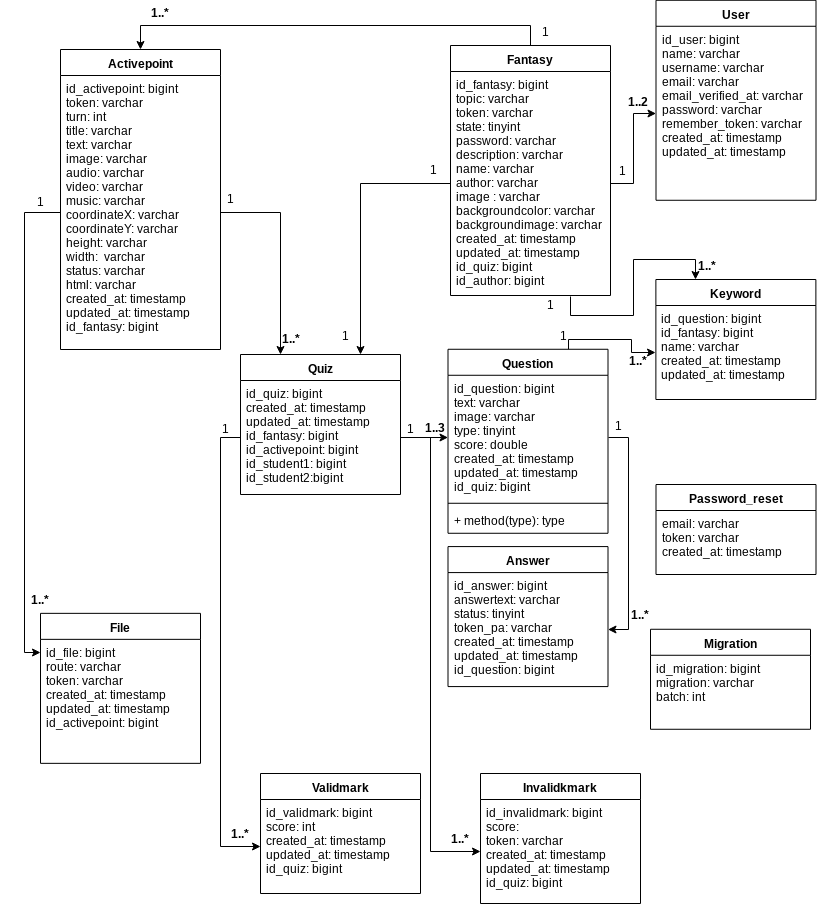
\includegraphics[scale=0.5]{Developing/StimeyUML.png}
	\caption{Stimey database.}
	\label{Stimey database}
\end{figure}

\section{Design of components}
The components used in the development of Fantasy project are: Laravel framework, MySQL and phpMyAdmin.

Thanks to this elements, we could incorporate the necesary views and controllers for the application functioning.

\section{Parameterization of the base software}
Not applicable.
	
	
\end{document}
